\documentclass[09pt,letterpaper]{article}
\usepackage[lmargin=2.2in,rmargin=0.7in,tmargin=1.0in,bmargin=1.0in]{geometry}
\usepackage{notes}
\begin{document}

\begin{center}
\Large\textbf{2.1 - Spring--Mass System (Unforced)}\\
\normalsize (Section 2.1)
\end{center}


%-------------------------------------------------------------
\section{Dimensional Analysis}

\subsection{Dimensions}
Physical constants and variables often have units, like the gravitational constant $g= 9.8 \,\mathrm{m/s^2}$. The \textbf{unit} is the standardized quantity in which the variable is measured. For the constant $g$, the units is meters per second squared. But more fundamentally, $g$ is described in length per unit of time squared. A \textbf{dimension} describes the type of physical quantity being measured, independent of the particular units used. In this sense, dimensions are generalized units. For example, meters, feet, and miles are all units of the dimension \textit{length}.

\subsection{Notation}
Many physical variables are composed of some combination of these global dimensions denoted by capital letters:
\begin{itemize}
    \item $L$: length
    \item $M$: mass
    \item $T$: time 
    \item $N$: quantity (like population)
    \item $\Theta$: temperature
    \item $1$: dimensionless
\end{itemize}
The full list of dimension letters is much longer, but we only use these for this class. We use bracket notation for expressing dimensions: 
$$
[ \text{ variable } ]  = \text{dimension of variable expressed in }L,M,T,\Theta, \text{etc}.
$$
For example, the dimensions of the gravitational constant is written
$$
[g] = LT^{-2}.$$ 
This indicates that $g$ is measured in length per unit time squared. If harvesting rate $h$ = 100 fish per month, then we write
$$[h]=NT^{-1}.$$ 

% Some variables are dimensionless. Typically, ratios and angles are dimensionless. Variables can be dimensionless but still have units. For example, $\theta=90\degree$ has units in degrees, but we write $[\theta]=1$.

\subsection{Dimension Rules}
Here are a few useful rules regarding dimensions:
\begin{enumerate}
    \item \textbf{Equality Rule}: The dimensions of both sides of an equation must match
    $$[\text{LHS}] = [\text{RHS}].$$
    \item \textbf{Multiplication Rule}: The dimension of a product is the product of the dimensions
    $$
    [x\,y] = [x][y]
    $$
    \item \textbf{Addition Rule}: You can only add variables with the same dimensions 
    $$
    x + y  \implies [x] = [y] 
    $$
    \item \textbf{Derivative Rule}: The dimension of a derivative is the quotient of the dimensions of the dependent and independent variables 
    $$
    \left[\frac{dx}{dt}\right] = \frac{[x]}{[t]}
    $$
    
    \item \textbf{Dimensionless Rule}: Quantities inside functions such as $\text{exp}(\cdot )$, $\ln(\cdot)$, and $\sin(\cdot)$ must be dimensionless. 
\end{enumerate}
We can use these rules to derive the dimensions of parameters in an equation. Here are a couple of examples.


\begin{example}[1]{
Newton's 2nd Law says force is $F=ma$, where $m$ is mass and $a$ is acceleration. Find the dimension of force.
}
\begin{align*}
    F &= ma&& \\
    [F] &= [ma]&&\com{equality rule}\\
    [F] &= [m][a] &&\com{multiplication rule}\\
    [F] &= MLT^{-2} &&\com{substitute}.
\end{align*}
The dimensions of force are 
$$
\boxed{[F] = MLT^{-2}.}
$$
\end{example}

Let's revisit one of the population models that we have studied.
\begin{example}[2]{
In the harvesting model $\frac{dP}{dt} = rP-h$, $P(t)$ represents the population at time $t$. Find the dimensions of $r$.
}
\begin{align*}
    \frac{dP}{dt} &= rP-h\\
    \left[\frac{dP}{dt}\right] &= [rP-h] &&\com{equality rule}\\
    NT^{-1} &= [rP-h] && \com{derivative rule}\\ 
    NT^{-1} &= [rP]=[h] && \com{addition rule}\\ 
    NT^{-1} &= [r][P] && \com{multiplication rule}\\
    NT^{-1} &= [r]N && \com{substitute}\\
    T^{-1} &= [r] &&\com{divide by $N$}\\
\end{align*}
In the last step, we divide both sides by $N$ to solve for $[r]$. The dimension of $r$ is
$$
\boxed{[r]=T^{-1}.}
$$
After substituting the global dimensions, you may use standard algebraic operations to solve for the dimension of the remaining parameter. 
\end{example}

%-------------------------------------------------------------

\section{Deriving the Spring Model}
In this section, we will derive a model for the movement of an object bouncing on a spring. This turns out to be a 2nd order DE. There are many types of springs (plastic springs, torsion springs, etc.). The type of spring we are interested in is the \textit{ideal linear spring}.

\subsection{Setup}
We will describe the setup for the \textit{simple spring oscillator} (horizontal version). There are two ways to describe the oscillator. One involves a spring dangling from the ceiling. We will do the setup where the mass is on a table. Both descriptions boil down to the same model.

Imagine a ball of mass $m$ lying on a table. The ball is connected to a rigid side wall by a spring. Initially, the mass is at equilibrium and the spring is neither stretched nor compressed. Let $x(t)$ be the position of the ball along the table. We will call the equilibrium position $x=0$. If the ball is to the right of the equilibrium, then $x>0$.   

The ball will not move on its own, so we must displace it from equilibrium to set it in motion. Suppose the ball is pulled to the right by a distance $x_0$, which causes the spring to stretch. This gives the ball potential energy. When the ball is let go, it will bounce back and forth along the table. We write the initial condition as 
$$ x(0)=x_0,\quad x'(0)=0.$$
The condition $x'(0)=0$ is used to indicate that the ball is released without adding any initial velocity. The goal is to write a model for the position $x(t)$.


\begin{figure}[H]
\centering
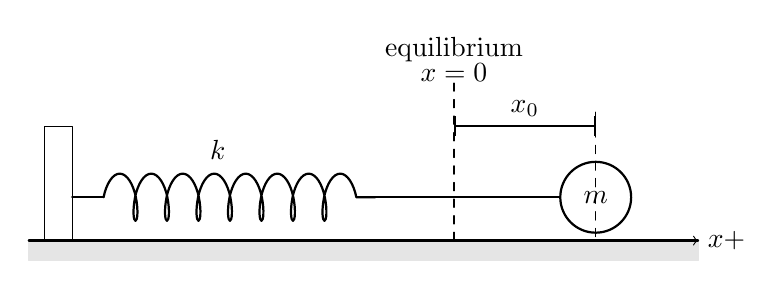
\begin{tikzpicture}[scale=1.0, line cap=round, line join=round]
\usetikzlibrary{decorations.pathmorphing}

% ----------------------------
% Parameters (tweak as needed)
% ----------------------------
\def\floorY{0}
\def\wallX{0}
\def\springL{4.2}      % spring start-to-end x-length
\def\eqX{5.2}          % equilibrium vertical line x-position
\def\massX{7.0}        % mass center x-position
\def\massR{0.45}       % mass radius
\def\tableH{0.25}      % table thickness
\def\springY{0.55}     % spring height above table top

% ----------------------------
% Table / ground
% ----------------------------
\draw[fill=gray!20, draw=gray!20]
(-0.2,\floorY-\tableH) -- (8.3,\floorY-\tableH) --
(8.3,\floorY) -- (-0.2,\floorY) -- cycle;

\draw[thick] (-0.2,\floorY) -- (8.3,\floorY);
\draw[->] (0,0) -- (8.3,0) node[right] {$x+$};

% ----------------------------
% Wall block
% ----------------------------
\draw
(\wallX,\floorY)
rectangle
(\wallX+0.35,\floorY+1.45);

% ----------------------------
% Spring
% ----------------------------

% lead-in segment
\draw[thick]
(\wallX+0.35,\springY)
--
(\wallX+0.75,\springY);

% coil
\draw[
    thick,
    decorate,
    decoration={
        coil,
        aspect=0.35,
        segment length=4mm,
        amplitude=3mm
    }
]
(\wallX+0.75,\springY)
--
(\wallX+\springL,\springY);

% lead-out segment
\draw[thick]
(\wallX+\springL,\springY)
--
(\massX-\massR,\springY);

% spring constant label
\node[above] at (\wallX+2.2,\springY+0.35) {$k$};

% ----------------------------
% Equilibrium dashed line + label
% ----------------------------
\draw[dashed] (\eqX,\floorY) -- (\eqX,2.0);

\node[above] at (\eqX,2.15) {equilibrium};
\node[above] at (\eqX,1.9) {$x=0$};

% ----------------------------
% Mass
% ----------------------------
\draw[thick,fill=white]
(\massX,\springY) circle (\massR);

\node at (\massX,\springY) {$m$};

% ----------------------------
% Displacement arrow x_0
% ----------------------------
\draw[dashed]
(\massX,\springY-\massR-0.05)
--
(\massX,\springY+\massR+0.65);

\draw[|-|,thick]
(\eqX,\springY+\massR+0.45)
--
(\massX,\springY+\massR+0.45);

\node[above]
at ({(\eqX+\massX)/2},\springY+\massR+0.45)
{$x_0$};

\end{tikzpicture}

\caption{
This is the setup for a horizontal spring oscillator.
The mass is pulled $x_0$ units to the right of equilibrium and then released.
}
\end{figure}

\subsection{Hooke's Law}
We assume that the spring attached to the ball is an \textit{ideal linear spring}. This means the spring has a restorative force that is proportional to the amount of compression or elongation. The spring wants to return the ball to the neutral position $x=0$. The forces exerted on the ball by the spring is given by \textbf{Hooke's Law}
$$F_s=-kx$$ for $k>0$. This equation captures both the pushing and pulling effects of the spring.
\begin{itemize}
    \item If the ball is to the right of the equilibrium, then $x>0$. Then $F_s=-kx <0$. A negative force indicates that the spring is pulling the ball to the left. This makes sense because the spring is in a stretched position and wants to contract to its original length.
    
    \item If the ball is to the left of the equilibrium, then $x<0$. Then $F_s=-kx >0$. A positive force indicates that the spring is pushing the ball to the right. This makes sense because the spring is in a contracted position and wants to extend back to its original length.
\end{itemize}


\subsection{Forces on the Mass}

Our goal is to use Newton's Second Law to derive an equation for $x(t)$. There are three forces acting on the mass:
\begin{enumerate}
    \item \textbf{Weight}: gravity pulls downward with magnitude $mg$.
    \item \textbf{Normal force}: the table pushes upward with equal magnitude $N=mg$.
    \item \textbf{Spring force}: the spring exerts the horizontal force
    \[
    F_s=-kx.
    \]
\end{enumerate}

The weight and normal force cancel, so the only force in the horizontal direction is the spring force. Newton's Second Law in the $x$-direction gives
\begin{align*}
\sum F_x &= m x''\\
-kx &= m x''.
\end{align*}
Therefore,
\[
m x''+kx=0.
\]
This is called the \textbf{spring-mass equation}. For the experiment described above, the complete model is
\[
\begin{dcases}
m x''+kx=0,\\
x(0)=x_0,\\
x'(0)=0.
\end{dcases}
\]
This is our first look at a \textit{second order differential equation}.

\subsection{Measuring the Spring Constant}

The constant $k$ is called the \textbf{spring constant} and measures the stiffness of the spring. The value of $k$ can be determined experimentally. Hang the spring vertically and attach a mass $m$ to its end. The weight causes the spring to stretch by a measurable distance $\Delta L$ from its unloaded length, as shown in Figure 2. Once the mass comes to rest, it is in equilibrium. There are two forces acting on the mass:
\begin{itemize}
    \item the downward weight $mg$,
    \item the upward spring force with magnitude $k\Delta L$.
\end{itemize}
Since the mass is stationary, Newton's Second Law gives
\begin{align*}
    \sum F &= 0,\\
    mg-k\Delta L &=0.
\end{align*}
Thus, by measuring the mass $m$ and the elongation $\Delta L$, we have enough information to determine the spring constant $k$.
\begin{figure}[H]  
\begin{center}
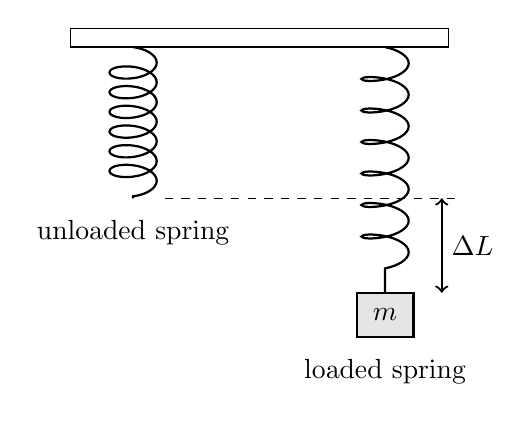
\begin{tikzpicture}[scale=0.8]
% ------------------------------------------------
% Parameters
% ------------------------------------------------
\def\xA{0}
\def\xB{4}
\def\ytop{4.5}
\def\Lzero{2.4}
\def\dL{1.5}
% ------------------------------------------------
% Ceiling
% ------------------------------------------------
\draw (-1,4.5) rectangle (5,4.8);
\draw[thick] (-1,4.5) -- (5,4.5);
% ------------------------------------------------
% Unloaded spring
% ------------------------------------------------
\draw[
    decorate,
    decoration={
        coil,
        aspect=0.45,
        segment length=2.5mm,
        amplitude=3mm
    },
    thick
]
(\xA,\ytop) -- (\xA,\ytop-\Lzero);

\node[below] at (\xA,\ytop-\Lzero-0.2)
{unloaded spring};
% ------------------------------------------------
% Loaded spring
% ------------------------------------------------
\draw[
    decorate,
    decoration={
        coil,
        aspect=0.35,
        segment length=4mm,
        amplitude=3mm
    },
    thick
]
(\xB,\ytop) -- (\xB,\ytop-\Lzero-\dL);

% Mass
\draw[thick,fill=gray!20]
(\xB-0.45,\ytop-\Lzero-\dL-0.7)
rectangle
(\xB+0.45,\ytop-\Lzero-\dL);

\node at (\xB,\ytop-\Lzero-\dL-0.35) {$m$};

\node[below] at (\xB,\ytop-\Lzero-\dL-0.9)
{loaded spring};

% ------------------------------------------------
% Reference line at natural length
% ------------------------------------------------
\draw[dashed]
(\xA+0.5,\ytop-\Lzero)
--
(\xB+1.2,\ytop-\Lzero);
% ------------------------------------------------
% Delta L
% ------------------------------------------------
\draw[<->,thick]
(\xB+0.9,\ytop-\Lzero)
--
(\xB+0.9,\ytop-\Lzero-\dL);

\node[right] at
(\xB+0.9,\ytop-\Lzero-0.5*\dL)
{$\Delta L$};
\end{tikzpicture}
\end{center}
\caption{Attaching a weight to the spring causes it to stretch by a measurable distance $\Delta L$.}
\end{figure}

%-------------------------------------------------------------

\section{Undamped vs. Damped}

There are two versions of the spring-mass model that we will study. The \textit{undamped} model ignores friction, while the \textit{damped} model includes friction. We will first examine the behavior of the undamped model and then see how friction changes the motion.


\subsection{Undamped Oscillator}

If the mass on the spring oscillator is pulled a distance $x_0$ from equilibrium and released from rest, then the model is 
\[
\begin{dcases}
    m\,x''=-k\,x,\\
    x(0)=x_0,\\
    x'(0)=0.
\end{dcases}
\]
Solving this IVP gives the position of the mass at any time $t$. We do not yet know how to solve this DE, so for now we will simply state the solution:
\[
x(t)=x_0\cos\left(\sqrt{\frac{k}{m}}\,t\right).
\]
We will learn how to derive this solution later in the course. Let's verify that the function satisfies the differential equation:
\[
\begin{aligned}
\text{LHS}&=m\,x''\\
           &=m\left(x_0 \cos(\sqrt{k/m}\,t)\right)''\\
           &=m\left(-x_0\sqrt{\frac{k}{m}}
             \sin(\sqrt{k/m}\,t)\right)'\\
           &=m\left(-x_0\frac{k}{m}
             \cos(\sqrt{k/m}\,t)\right)\\
           &=-x_0k\cos(\sqrt{k/m}\,t),
\end{aligned}
\qquad
\begin{aligned}
\text{RHS}&=-k\,x\\
           &=-k\left(x_0\cos(\sqrt{k/m}\,t)\right)\\
           &=\text{LHS}.
\end{aligned}
\]
You can also check that the function satisfies the two initial conditions.

This motion is called an \textbf{undamped oscillator}. The word ``undamped'' means that no friction or other resistance is removing energy from the system.


\subsection{Plotting the Solution}
We can understand the motion by plotting
\[
x(t)=x_0\cos\left(\sqrt{\frac{k}{m}}\,t\right).
\]
There are three important features of the solution:
\begin{enumerate}
    \item \textbf{Amplitude}: The mass oscillates between $x=-x_0$ and $x=x_0$.
    
    \item \textbf{Period}: The motion repeats every
    \[
    T=2\pi\sqrt{\frac{m}{k}}
    \]
    units of time.
    
    \item \textbf{Initial position}: At $t=0$, the mass begins at $x=x_0$.
\end{enumerate}

\begin{figure}[H]
\centering
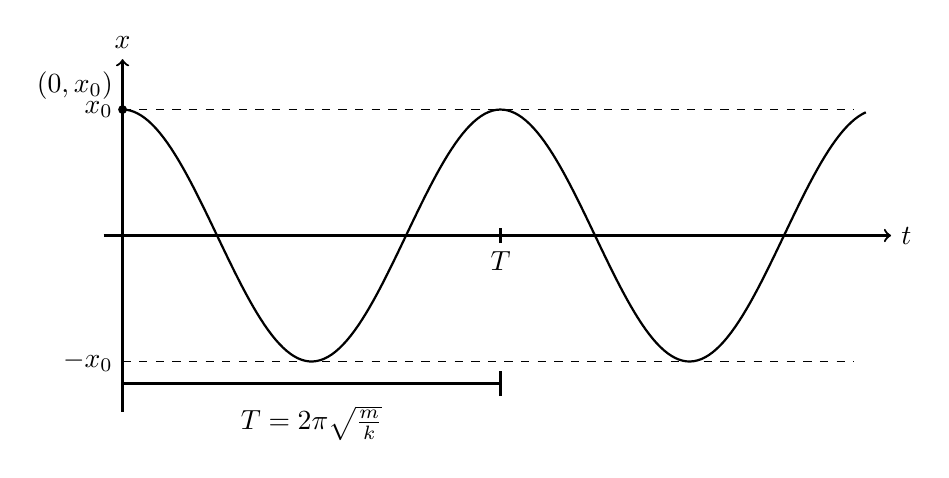
\begin{tikzpicture}[scale=0.8]
    %-----------------------------
    % Parameters for the picture
    %-----------------------------
    \def\A{2.0}        % amplitude = x0 (in picture units)
    \def\T{6.0}        % one period length (in picture units)
    \def\xMax{12.2}     % right end of t-axis
    \def\yMax{2.8}     % top of x-axis
    \def\yMin{-2.8}    % bottom of x-axis
    \def\w{360/\T}     % degrees per unit t so that period = T

    % Axes
    \draw[->,thick] (-0.3,0) -- (\xMax,0) node[right] {$t$};
    \draw[->,thick] (0,\yMin) -- (0,\yMax) node[above] {$x$};

    % Cosine solution: x(t)=x0 cos(2pi t / T)
    \draw[thick,domain=0:\xMax-0.4,samples=200]
        plot (\x,{\A*cos(\w*\x)});

    % Amplitude dashed lines (optional but usually helpful)
    \draw[dashed] (0,\A) -- (\xMax-0.6,\A);
    \draw[dashed] (0,-\A) -- (\xMax-0.6,-\A);
    \node[left] at (0,\A) {$x_0$};
    \node[left] at (0,-\A) {$-x_0$};

    % Mark initial condition point (0,x0)
    \fill (0,\A) circle (2pt);
    \node[above left] at (0,\A) {$(0,x_0)$};

    % Period bracket: |-| over one period [0,T]
    \draw[thick] (0,-2.35) -- (\T,-2.35);
    \draw[thick] (0,-2.55) -- (0,-2.15);
    \draw[thick] (\T,-2.55) -- (\T,-2.15);
    \node[below] at (\T/2,-2.55) {$T=2\pi\sqrt{\frac{m}{k}}$};

    % Tick at T (optional)
    \draw[thick] (\T,-0.12) -- (\T,0.12);
    \node[below] at (\T,-0.1) {$T$};
\end{tikzpicture}
\caption{Solution curve $x(t)=x_0\cos\!\bigl(\sqrt{k/m}\,t\bigr)$ showing amplitude, period, and initial condition.}
\end{figure}

The model predicts that the mass will oscillate between $-x_0$ and $x_0$ forever. This is not realistic. In a physical spring-mass system, the initial energy eventually dissipates, and the oscillations die out. What is missing from our model? We assumed that there was no friction. To obtain a more realistic model, we need to include a force that resists the motion of the mass.

\subsection{Damped Oscillator}
To make our model more realistic, we need to account for friction. As the ball slides across the table, it should feel a resistive force in the direction opposite to its movement. We model the \textbf{damping force} as
\[
F_{\text{d}} = -\gamma\,x'(t),
\qquad \gamma>0.
\]
This equation states that the faster an object moves, the more resistance it feels.

There are now two horizontal forces acting on the mass: the spring force $F_s=-kx$ and the damping force $F_d=-\gamma x'$. Newton's Second Law gives
\[
m x'' + \gamma x' + kx = 0\,.
\]
We call this the \textbf{damped oscillator equation}.
We do not yet know how to solve this equation. Depending on the amount of damping, its solutions can behave in different ways. We will study these different cases later in the course. For now, the important idea is that damping causes the motion to die out over time. In particular,
\[
\lim_{t\to\infty}x(t)=0.
\]
Thus, unlike the undamped oscillator, the mass eventually approaches its equilibrium position.

\subsection{Plotting a Damped Oscillation}
If the damping is not too strong, the mass will continue to oscillate while gradually losing energy. A typical solution has the form
\[
x(t)=Ae^{-\lambda t}\cos(\omega t),
\qquad \lambda>0.
\]
We will derive this solution later. For now, we can use it to understand what damping does to the motion.

The cosine factor produces the oscillation, while the exponential factor
\[
e^{-\lambda t}
\]
causes its amplitude to decrease over time. There are three important features of the graph:
\begin{enumerate}
    \item \textbf{Envelopes}: Since $-1\leq \cos(\omega t)\leq 1$, the solution is trapped between
    \[
    -Ae^{-\lambda t}
    \qquad\text{and}\qquad
    Ae^{-\lambda t}.
    \]
    These curves are called the \textbf{envelopes} of the oscillation.

    \item \textbf{Quasiperiod}: The solution is not truly periodic because its amplitude is constantly decreasing. However, successive peaks are separated by
    \[
    T=\frac{2\pi}{\omega}.
    \]
    We call $T$ the \textbf{quasiperiod}.

    \item \textbf{Initial conditions}: The initial condition tells us where the solution curve must begin. If
    \[
    x(0)=x_0,
    \]
    then the graph must pass through the point $(0,x_0)$. The initial velocity
    $$
    x'(0)=v_0
    $$
    tells us the slope of the solution curve in the beginning.
\end{enumerate}

\begin{figure}[H]
\centering
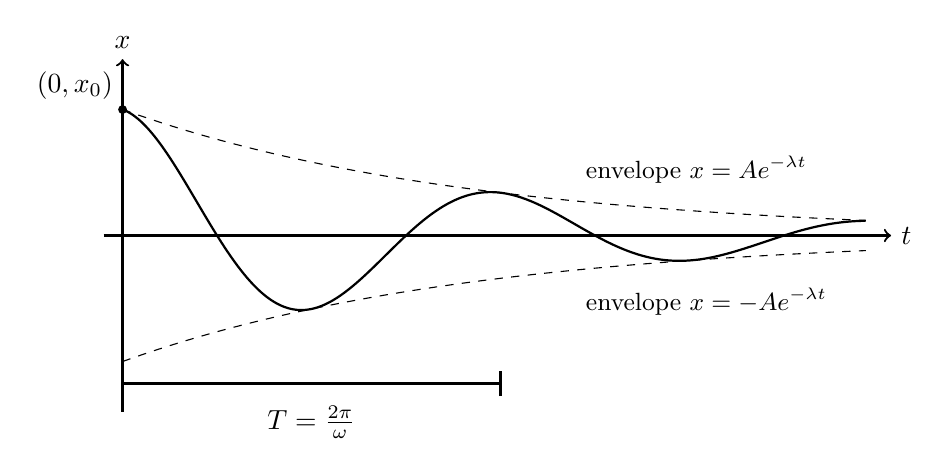
\begin{tikzpicture}[scale=0.8]
    %-----------------------------
    % Parameters (picture only)
    %-----------------------------
    \def\A{2.0}          % initial amplitude
    \def\T{6.0}        % one period length (in picture units)
    \def\gam{0.18}       % decay rate (envelope)
    \def\om{180/3}       % degrees per unit t (roughly period ~3)
    \def\xMax{12.2}
    \def\yMax{2.8}
    \def\yMin{-2.8}

    % Axes
    \draw[->,thick] (-0.3,0) -- (\xMax,0) node[right] {$t$};
    \draw[->,thick] (0,\yMin) -- (0,\yMax) node[above] {$x$};

    % Damped oscillation: A e^{-gam t} cos(om t)
    \draw[thick,domain=0:\xMax-0.4,samples=350]
        plot (\x,{\A*exp(-\gam*\x)*cos(\om*\x)});

    % Envelopes: ±A e^{-gam t}
    \draw[dashed,domain=0:\xMax-0.4,samples=150]
        plot (\x,{\A*exp(-\gam*\x)});
    \draw[dashed,domain=0:\xMax-0.4,samples=150]
        plot (\x,{-\A*exp(-\gam*\x)});

    % Initial condition point (0,x0)
    \fill (0,\A) circle (2pt);
    \node[above left] at (0,\A) {$(0,x_0)$};

    % Label the envelope
    \node[right] at (7.2,1.05) {\small envelope $x=A e^{-\lambda t}$};
    \node[right] at (7.2,-1.05) {\small envelope $x=-A e^{-\lambda t}$};

        % Period bracket: |-| over one period [0,T]
    \draw[thick] (0,-2.35) -- (\T,-2.35);
    \draw[thick] (0,-2.55) -- (0,-2.15);
    \draw[thick] (\T,-2.55) -- (\T,-2.15);
    \node[below] at (\T/2,-2.55) {$T={\frac{2\pi}{\omega}}$};
\end{tikzpicture}
\caption{Damped oscillation: the amplitude decays over time due to friction.}
\end{figure}


%-------------------------------------------------------------
\section{Energy in a System}
We can also understand the behavior of the spring-mass model through the concept of energy. Energy gives us another way to explain why the undamped oscillator continues forever while the damped oscillator eventually comes to rest.


\subsection{Informal Definitions}

We will only need an informal understanding of energy in this class. A \textbf{system} refers to the objects that we are studying. For the spring-mass model, the system consists of the spring and the mass. The \textbf{environment} is everything outside of the system, such as the table and the surrounding air.

\textbf{Energy} is the ability of a system to produce motion or change. Energy can move between different forms within the system, and it can also be transferred from the system to its environment.

\subsection{Types of Energy}

For the spring-mass system, we are interested in two forms of mechanical energy: \textit{kinetic energy} and \textit{potential energy}.

\textbf{Kinetic energy} is the energy associated with motion:
\[
T=\frac12 m(x')^2.
\]
The faster the mass moves, the more kinetic energy it has. \textbf{Potential energy} is energy stored in the spring due to its displacement from equilibrium:
\[
V=\frac12 kx^2.
\]
The farther the spring is stretched or compressed, the more potential energy it stores. Finally, the \textbf{total mechanical energy} of the system is the sum
\[
E=T+V
  =\frac12 m(x')^2+\frac12 kx^2.
\]
Since both terms depend on $x(t)$ and $x'(t)$, the total energy $E(t)$ may change with time. Also, since $T\geq0$ and $V\geq0$, we always have $E\geq0$.

\subsection{Energy in the Damped Oscillator}

Consider the damped oscillator
\[
mx''+\gamma x'+kx=0.
\]
Multiply the equation by the velocity $x'$:
\[
mx'x''+\gamma(x')^2+kxx'=0.
\]
Using the chain rule in reverse,
\[
x'x''=\frac12\frac{d}{dt}(x')^2,
\qquad
xx'=\frac12\frac{d}{dt}x^2.
\]
Therefore,
\begin{align*}
mx'x''+\gamma(x')^2+kxx'&=0\\
\frac{d}{dt}\left(\frac12m(x')^2\right)
+\gamma(x')^2
+\frac{d}{dt}\left(\frac12kx^2\right)&=0\\
\frac{d}{dt}\left(
\frac12m(x')^2+\frac12kx^2
\right)&=-\gamma(x')^2\\
E'(t)&=-\gamma(x')^2.
\end{align*}

Since $\gamma>0$ and $(x')^2\geq0$,
\[
E'(t)\leq0.
\]
Thus, the total mechanical energy can never increase. Whenever the mass is moving, $x'\neq0$ and therefore $E'(t)<0$. Energy is being transferred out of the spring-mass system through damping. The energy is converted to heat or sound. This explains why the oscillations become smaller over time. Energy leaves the system, and never returns. The mass eventually approaches the equilibrium position. \\

\noindent Suppose we assume there is no friction. How would the total mechanical energy change?
\end{document}
